% Options for packages loaded elsewhere
\PassOptionsToPackage{unicode}{hyperref}
\PassOptionsToPackage{hyphens}{url}
%
\documentclass[
  man]{apa6}
\usepackage{amsmath,amssymb}
\usepackage{lmodern}
\usepackage{iftex}
\ifPDFTeX
  \usepackage[T1]{fontenc}
  \usepackage[utf8]{inputenc}
  \usepackage{textcomp} % provide euro and other symbols
\else % if luatex or xetex
  \usepackage{unicode-math}
  \defaultfontfeatures{Scale=MatchLowercase}
  \defaultfontfeatures[\rmfamily]{Ligatures=TeX,Scale=1}
\fi
% Use upquote if available, for straight quotes in verbatim environments
\IfFileExists{upquote.sty}{\usepackage{upquote}}{}
\IfFileExists{microtype.sty}{% use microtype if available
  \usepackage[]{microtype}
  \UseMicrotypeSet[protrusion]{basicmath} % disable protrusion for tt fonts
}{}
\makeatletter
\@ifundefined{KOMAClassName}{% if non-KOMA class
  \IfFileExists{parskip.sty}{%
    \usepackage{parskip}
  }{% else
    \setlength{\parindent}{0pt}
    \setlength{\parskip}{6pt plus 2pt minus 1pt}}
}{% if KOMA class
  \KOMAoptions{parskip=half}}
\makeatother
\usepackage{xcolor}
\usepackage{longtable,booktabs,array}
\usepackage{calc} % for calculating minipage widths
% Correct order of tables after \paragraph or \subparagraph
\usepackage{etoolbox}
\makeatletter
\patchcmd\longtable{\par}{\if@noskipsec\mbox{}\fi\par}{}{}
\makeatother
% Allow footnotes in longtable head/foot
\IfFileExists{footnotehyper.sty}{\usepackage{footnotehyper}}{\usepackage{footnote}}
\makesavenoteenv{longtable}
\usepackage{graphicx}
\makeatletter
\def\maxwidth{\ifdim\Gin@nat@width>\linewidth\linewidth\else\Gin@nat@width\fi}
\def\maxheight{\ifdim\Gin@nat@height>\textheight\textheight\else\Gin@nat@height\fi}
\makeatother
% Scale images if necessary, so that they will not overflow the page
% margins by default, and it is still possible to overwrite the defaults
% using explicit options in \includegraphics[width, height, ...]{}
\setkeys{Gin}{width=\maxwidth,height=\maxheight,keepaspectratio}
% Set default figure placement to htbp
\makeatletter
\def\fps@figure{htbp}
\makeatother
\setlength{\emergencystretch}{3em} % prevent overfull lines
\providecommand{\tightlist}{%
  \setlength{\itemsep}{0pt}\setlength{\parskip}{0pt}}
\setcounter{secnumdepth}{-\maxdimen} % remove section numbering
% Make \paragraph and \subparagraph free-standing
\ifx\paragraph\undefined\else
  \let\oldparagraph\paragraph
  \renewcommand{\paragraph}[1]{\oldparagraph{#1}\mbox{}}
\fi
\ifx\subparagraph\undefined\else
  \let\oldsubparagraph\subparagraph
  \renewcommand{\subparagraph}[1]{\oldsubparagraph{#1}\mbox{}}
\fi
\newlength{\cslhangindent}
\setlength{\cslhangindent}{1.5em}
\newlength{\csllabelwidth}
\setlength{\csllabelwidth}{3em}
\newlength{\cslentryspacingunit} % times entry-spacing
\setlength{\cslentryspacingunit}{\parskip}
\newenvironment{CSLReferences}[2] % #1 hanging-ident, #2 entry spacing
 {% don't indent paragraphs
  \setlength{\parindent}{0pt}
  % turn on hanging indent if param 1 is 1
  \ifodd #1
  \let\oldpar\par
  \def\par{\hangindent=\cslhangindent\oldpar}
  \fi
  % set entry spacing
  \setlength{\parskip}{#2\cslentryspacingunit}
 }%
 {}
\usepackage{calc}
\newcommand{\CSLBlock}[1]{#1\hfill\break}
\newcommand{\CSLLeftMargin}[1]{\parbox[t]{\csllabelwidth}{#1}}
\newcommand{\CSLRightInline}[1]{\parbox[t]{\linewidth - \csllabelwidth}{#1}\break}
\newcommand{\CSLIndent}[1]{\hspace{\cslhangindent}#1}
\ifLuaTeX
\usepackage[bidi=basic]{babel}
\else
\usepackage[bidi=default]{babel}
\fi
\babelprovide[main,import]{english}
% get rid of language-specific shorthands (see #6817):
\let\LanguageShortHands\languageshorthands
\def\languageshorthands#1{}
% Manuscript styling
\usepackage{upgreek}
\captionsetup{font=singlespacing,justification=justified}

% Table formatting
\usepackage{longtable}
\usepackage{lscape}
% \usepackage[counterclockwise]{rotating}   % Landscape page setup for large tables
\usepackage{multirow}		% Table styling
\usepackage{tabularx}		% Control Column width
\usepackage[flushleft]{threeparttable}	% Allows for three part tables with a specified notes section
\usepackage{threeparttablex}            % Lets threeparttable work with longtable

% Create new environments so endfloat can handle them
% \newenvironment{ltable}
%   {\begin{landscape}\begin{center}\begin{threeparttable}}
%   {\end{threeparttable}\end{center}\end{landscape}}
\newenvironment{lltable}{\begin{landscape}\begin{center}\begin{ThreePartTable}}{\end{ThreePartTable}\end{center}\end{landscape}}

% Enables adjusting longtable caption width to table width
% Solution found at http://golatex.de/longtable-mit-caption-so-breit-wie-die-tabelle-t15767.html
\makeatletter
\newcommand\LastLTentrywidth{1em}
\newlength\longtablewidth
\setlength{\longtablewidth}{1in}
\newcommand{\getlongtablewidth}{\begingroup \ifcsname LT@\roman{LT@tables}\endcsname \global\longtablewidth=0pt \renewcommand{\LT@entry}[2]{\global\advance\longtablewidth by ##2\relax\gdef\LastLTentrywidth{##2}}\@nameuse{LT@\roman{LT@tables}} \fi \endgroup}

% \setlength{\parindent}{0.5in}
% \setlength{\parskip}{0pt plus 0pt minus 0pt}

% \usepackage{etoolbox}
\makeatletter
\patchcmd{\HyOrg@maketitle}
  {\section{\normalfont\normalsize\abstractname}}
  {\section*{\normalfont\normalsize\abstractname}}
  {}{\typeout{Failed to patch abstract.}}
\patchcmd{\HyOrg@maketitle}
  {\section{\protect\normalfont{\@title}}}
  {\section*{\protect\normalfont{\@title}}}
  {}{\typeout{Failed to patch title.}}
\makeatother
\shorttitle{Inflammation, Access to care, and Treatment among Older Mexicans with Diabetes}
\keywords{Diabetes, access to care, inflammation, health, Mexico, China\newline\indent Word count: X (this cannot easily be done automatically, we can also just leave it out)}
\DeclareDelayedFloatFlavor{ThreePartTable}{table}
\DeclareDelayedFloatFlavor{lltable}{table}
\DeclareDelayedFloatFlavor*{longtable}{table}
\makeatletter
\renewcommand{\efloat@iwrite}[1]{\immediate\expandafter\protected@write\csname efloat@post#1\endcsname{}}
\makeatother
\usepackage{csquotes}
\usepackage[titles]{tocloft}
\cftpagenumbersoff{figure}
\renewcommand{\cftfigpresnum}{\itshape\figurename\enspace}
\renewcommand{\cftfigaftersnum}{.\space}
\setlength{\cftfigindent}{0pt}
\setlength{\cftafterloftitleskip}{0pt}
\settowidth{\cftfignumwidth}{Figure 10.\qquad}
\cftpagenumbersoff{table}
\renewcommand{\cfttabpresnum}{\itshape\tablename\enspace}
\renewcommand{\cfttabaftersnum}{.\space}
\setlength{\cfttabindent}{0pt}
\setlength{\cftafterloftitleskip}{0pt}
\settowidth{\cfttabnumwidth}{Table 10.\qquad}
\ifLuaTeX
  \usepackage{selnolig}  % disable illegal ligatures
\fi
\IfFileExists{bookmark.sty}{\usepackage{bookmark}}{\usepackage{hyperref}}
\IfFileExists{xurl.sty}{\usepackage{xurl}}{} % add URL line breaks if available
\urlstyle{same} % disable monospaced font for URLs
\hypersetup{
  pdftitle={Relations between Inflammation and Access to care, Treatment, and Diabetes in Older Mexicans},
  pdfauthor={Dominik Grätz1, Rachel Miller-Moudgil1, Amber Somarriba1, Brittany Spinner1, \& Tian Walker1},
  pdflang={en-EN},
  pdfkeywords={Diabetes, access to care, inflammation, health, Mexico, China},
  hidelinks,
  pdfcreator={LaTeX via pandoc}}

\title{Relations between Inflammation and Access to care, Treatment, and Diabetes in Older Mexicans}
\author{Dominik Grätz\textsuperscript{1}, Rachel Miller-Moudgil\textsuperscript{1}, Amber Somarriba\textsuperscript{1}, Brittany Spinner\textsuperscript{1}, \& Tian Walker\textsuperscript{1}}
\date{}


\authornote{List of group members ordered by alphabet.}

\affiliation{\vspace{0.5cm}\textsuperscript{1} University of Oregon}

\abstract{
Diabetes is a leading cause of death in Mexico and is closely linked to the obesity epidemic. Previous studies indicate that inflammation predicts the development of diabetes and is found to be a strong indicator of diabetes development and progression. However, there are limited studies investigating the extent to which inflammation levels relate to the different treatment options among those with diabetes among Mexicans. To gain insight on the extent to which inflammation levels relate to medication, diet, and exercise we conducted a cross-sectional, secondary analysis using linear regression modeling and Chi-square tests of independence. Medication model fit parameter included (N = 357) F(2,354) = 1.06, p= 0.35, with R2= 0.01. Diet and exercise model fit parameters included (N= ) F(2, 354) = 2.70,p= 0.07 withR2= 0.02. And evaluating diet and exercise with access to care results included X2 results: X2(1) = 0.57, p= 0.45. Results indicate that among older Mexicans with diabetes there were no direct effects of treatment and access to inflammation levels.
}



\begin{document}
\maketitle

\begin{figure}
\centering
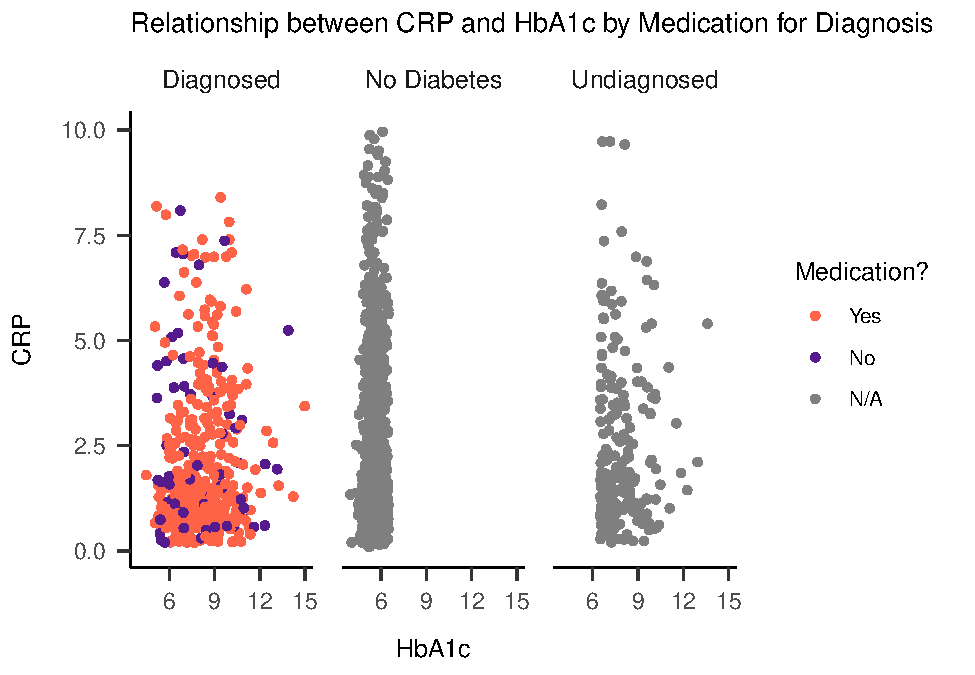
\includegraphics{NEW_Final_Groupof5_files/figure-latex/plot-all-1.pdf}
\caption{\label{fig:plot-all}Figure caption goes here.}
\end{figure}



\begin{figure}
\centering
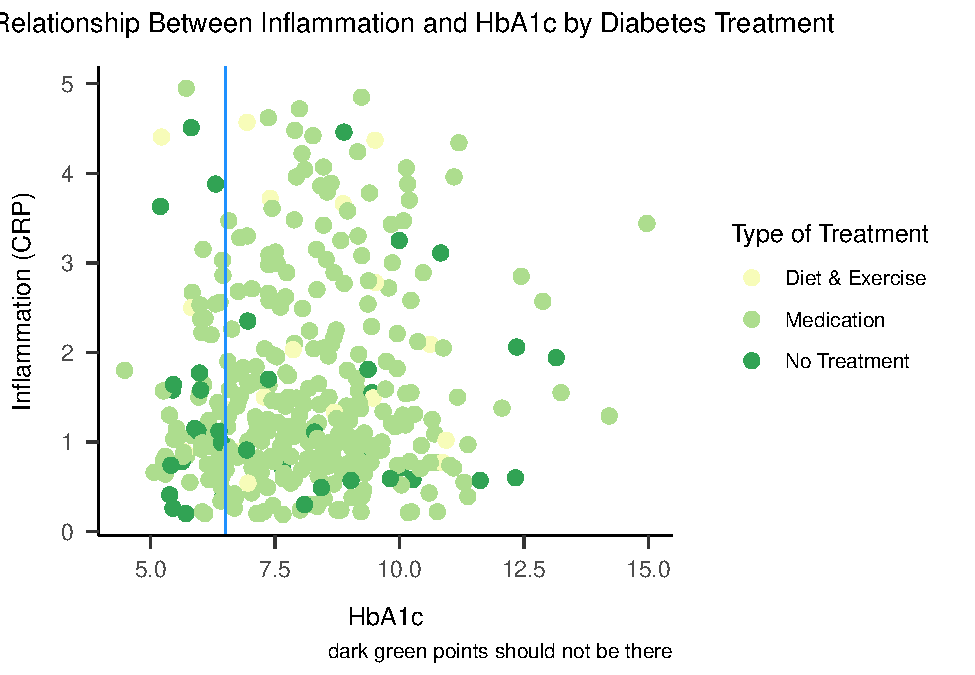
\includegraphics{NEW_Final_Groupof5_files/figure-latex/plot-all2-1.pdf}
\caption{\label{fig:plot-all2}Figure caption goes here.}
\end{figure}



\begin{figure}
\centering
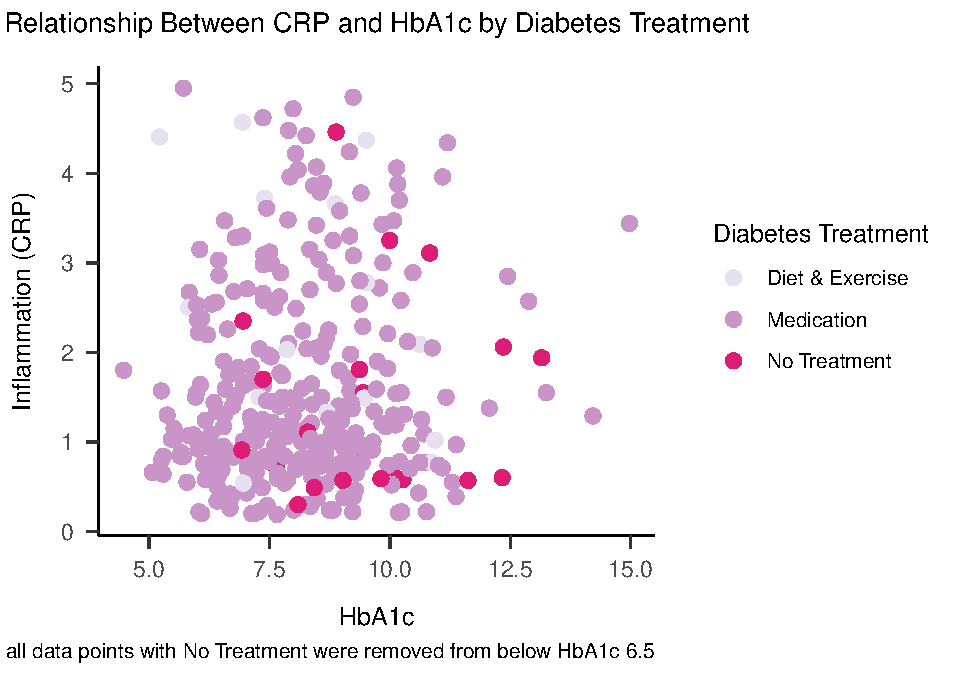
\includegraphics{NEW_Final_Groupof5_files/figure-latex/tian-fig-hba1c-65-1.pdf}
\caption{\label{fig:tian-fig-hba1c-65}Here goes the caption.}
\end{figure}



\begin{figure}
\centering
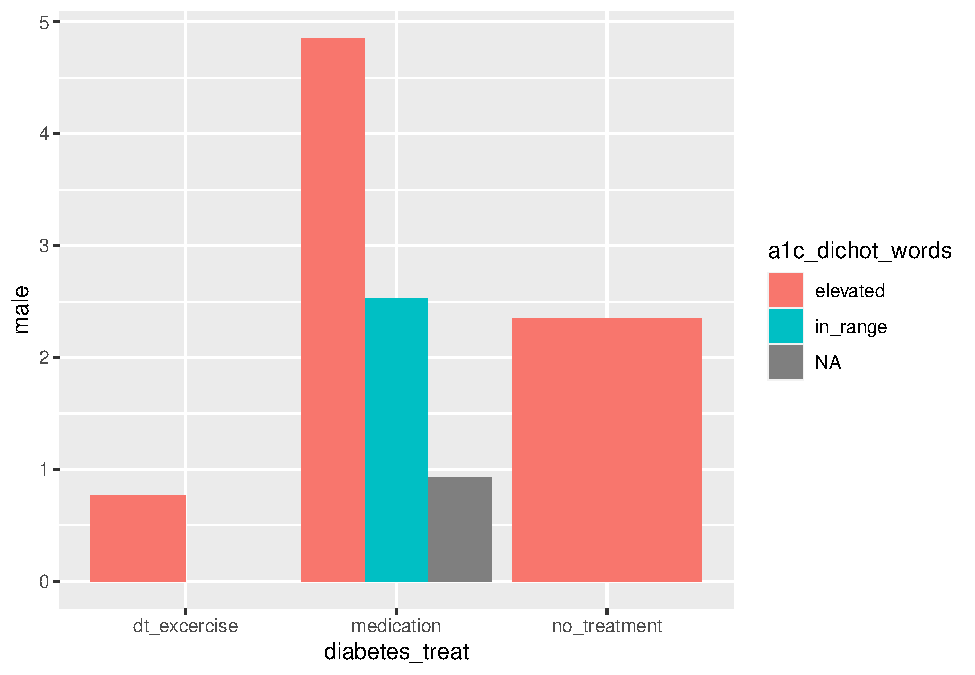
\includegraphics{NEW_Final_Groupof5_files/figure-latex/crp-by-sex-male-1.pdf}
\caption{\label{fig:crp-by-sex-male}Here goes the caption.}
\end{figure}



\begin{figure}
\centering
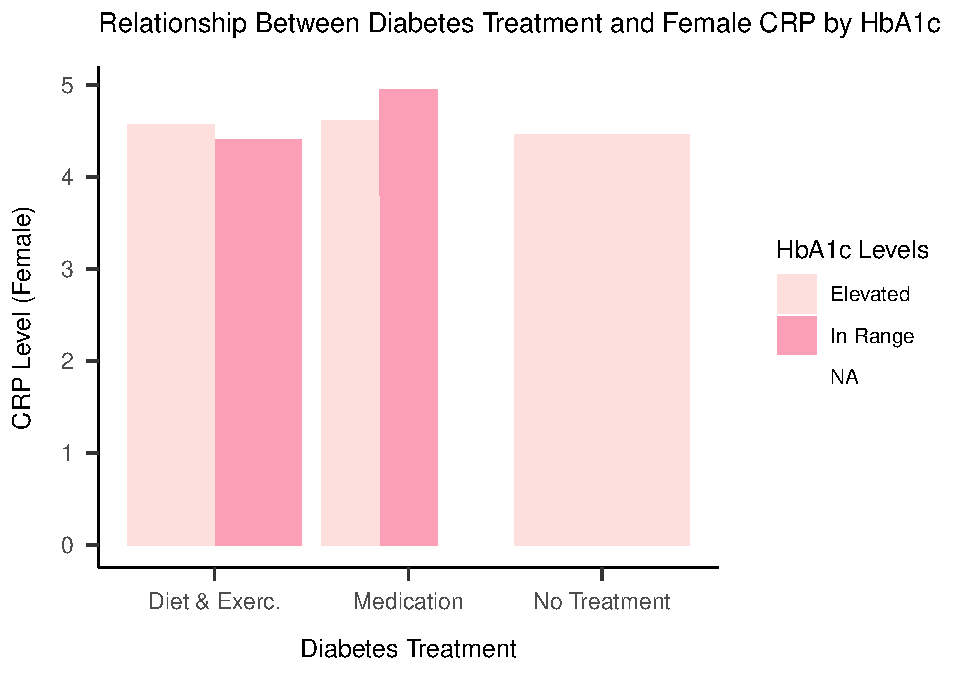
\includegraphics{NEW_Final_Groupof5_files/figure-latex/crp-by-sex-female-1.pdf}
\caption{\label{fig:crp-by-sex-female}Here goes the caption.}
\end{figure}



\begin{figure}
\centering
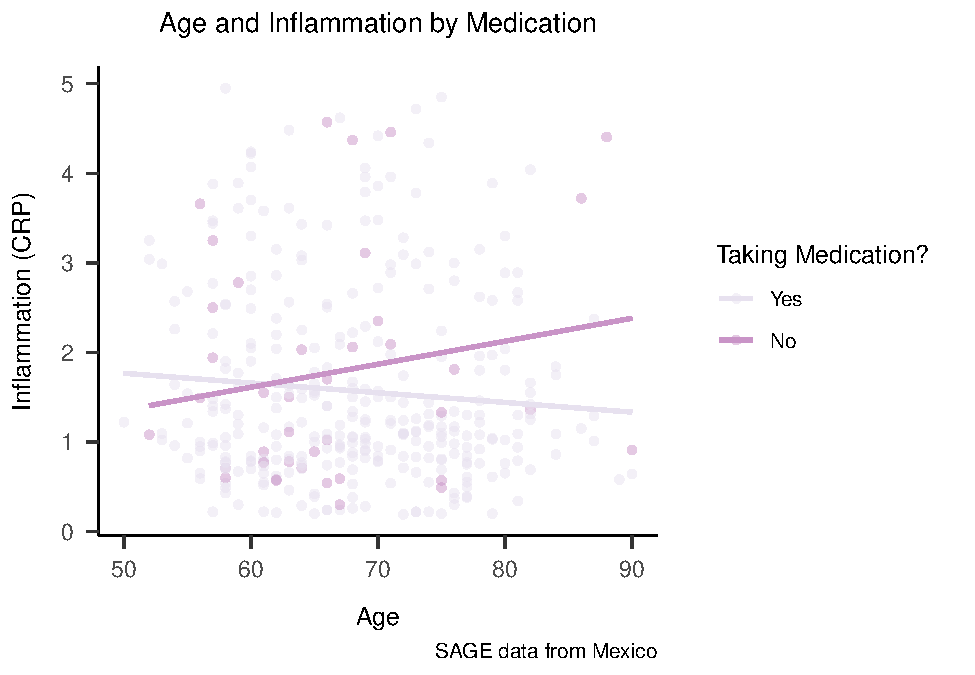
\includegraphics{NEW_Final_Groupof5_files/figure-latex/RQ1plot-1.pdf}
\caption{\label{fig:RQ1plot}Here goes the caption.}
\end{figure}



\begin{figure}
\centering
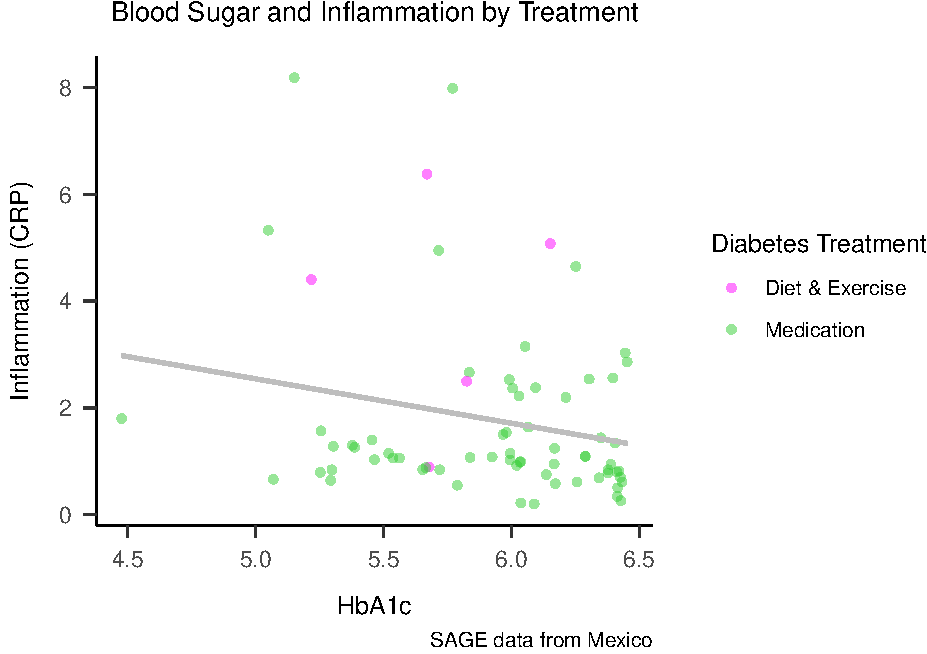
\includegraphics{NEW_Final_Groupof5_files/figure-latex/tian-filtering-1.pdf}
\caption{\label{fig:tian-filtering}Here goes the caption.}
\end{figure}



\begin{table}[tbp]

\begin{center}
\begin{threeparttable}

\caption{\label{tab:regtab1}Effect of Medication on CRP, controlling for Age. }

\begin{tabular}{lllll}
\toprule
Predictor & \multicolumn{1}{c}{$b$} & \multicolumn{1}{c}{95\% CI} & \multicolumn{1}{c}{$t(354)$} & \multicolumn{1}{c}{$p$}\\
\midrule
Intercept & 2.00 & $[1.06$, $2.94]$ & 4.18 & < .001\\
Age & -0.01 & $[-0.02$, $0.01]$ & -0.91 & .362\\
Medication & 0.20 & $[-0.17$, $0.56]$ & 1.07 & .284\\
\bottomrule
\addlinespace
\end{tabular}

\begin{tablenotes}[para]
\normalsize{\textit{Note.} Model fit: $F$(2, 354) = 1.06, $p$ = 0.35, $R^2$ = 0.01.}
\end{tablenotes}

\end{threeparttable}
\end{center}

\end{table}

\begin{table}[tbp]

\begin{center}
\begin{threeparttable}

\caption{\label{tab:RQ2}Effect of Diet and Exercise on CRP, controlling for Age.}

\begin{tabular}{lllll}
\toprule
Predictor & \multicolumn{1}{c}{$b$} & \multicolumn{1}{c}{95\% CI} & \multicolumn{1}{c}{$t(354)$} & \multicolumn{1}{c}{$p$}\\
\midrule
Intercept & 2.10 & $[1.17$, $3.04]$ & 4.43 & < .001\\
Age & -0.01 & $[-0.02$, $0.01]$ & -0.83 & .408\\
Diet and Exercise & -0.25 & $[-0.47$, $-0.02]$ & -2.11 & .036\\
\bottomrule
\addlinespace
\end{tabular}

\begin{tablenotes}[para]
\normalsize{\textit{Note.} Model fit: $F$(2, 354) = 2.71, $p$ = 0.07, $R^2$ = 0.02.}
\end{tablenotes}

\end{threeparttable}
\end{center}

\end{table}

\begin{figure}
\centering
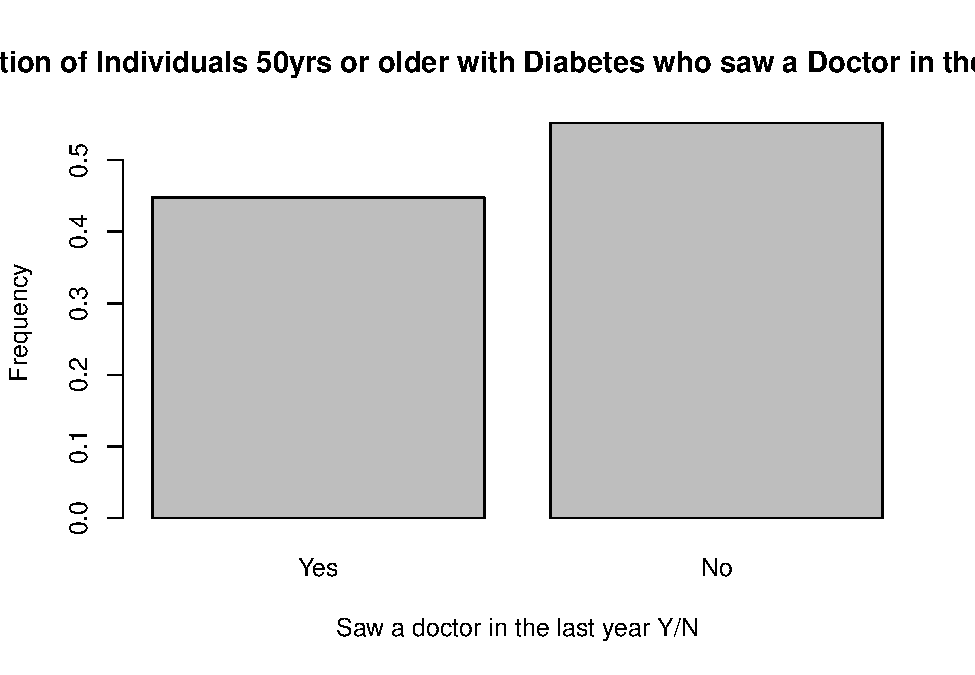
\includegraphics{NEW_Final_Groupof5_files/figure-latex/RQ3-brittany-1.pdf}
\caption{\label{fig:RQ3-brittany}Here goes the caption.}
\end{figure}



\begin{figure}
\centering
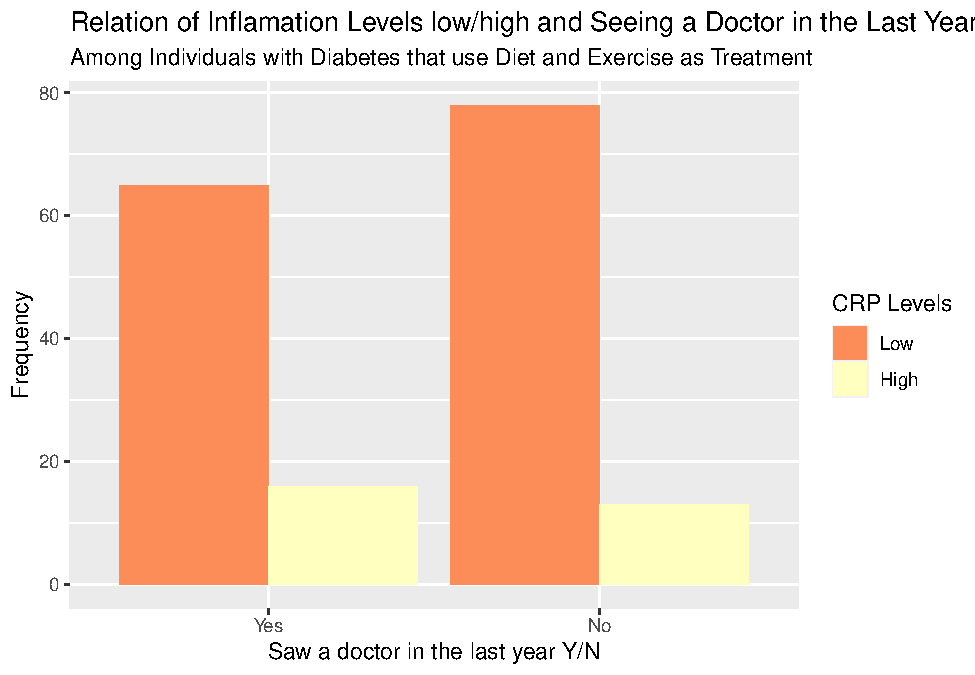
\includegraphics{NEW_Final_Groupof5_files/figure-latex/prop-access-bar-1.pdf}
\caption{\label{fig:prop-access-bar}Here goes the caption.}
\end{figure}



\begin{figure}
\centering
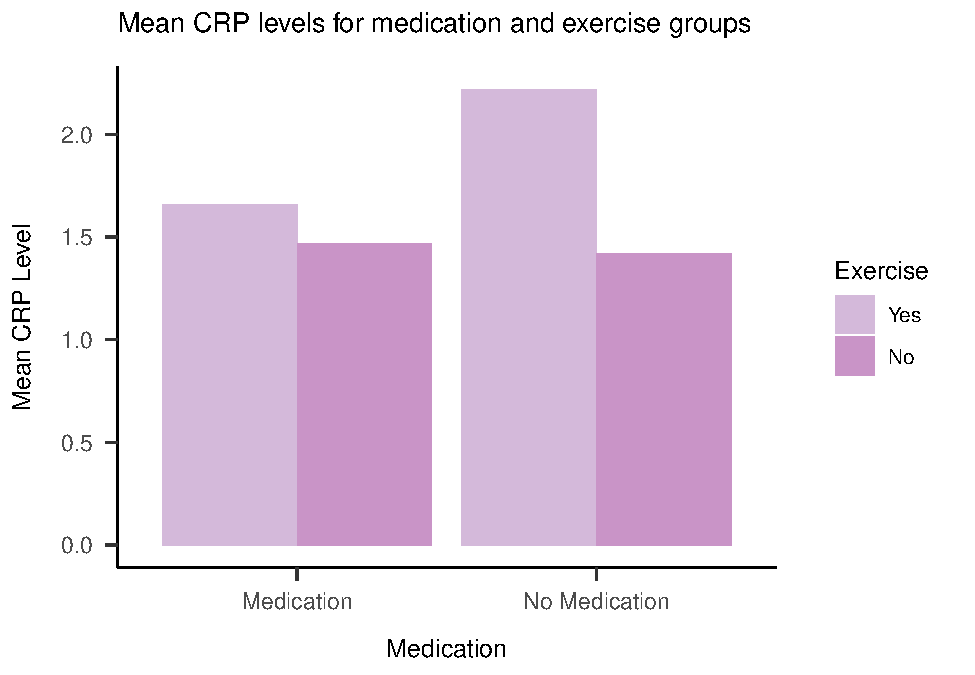
\includegraphics{NEW_Final_Groupof5_files/figure-latex/tableofcrpmedicationandexercise-1.pdf}
\caption{\label{fig:tableofcrpmedicationandexercise}Here goes the caption.}
\end{figure}

\begin{figure}
\centering
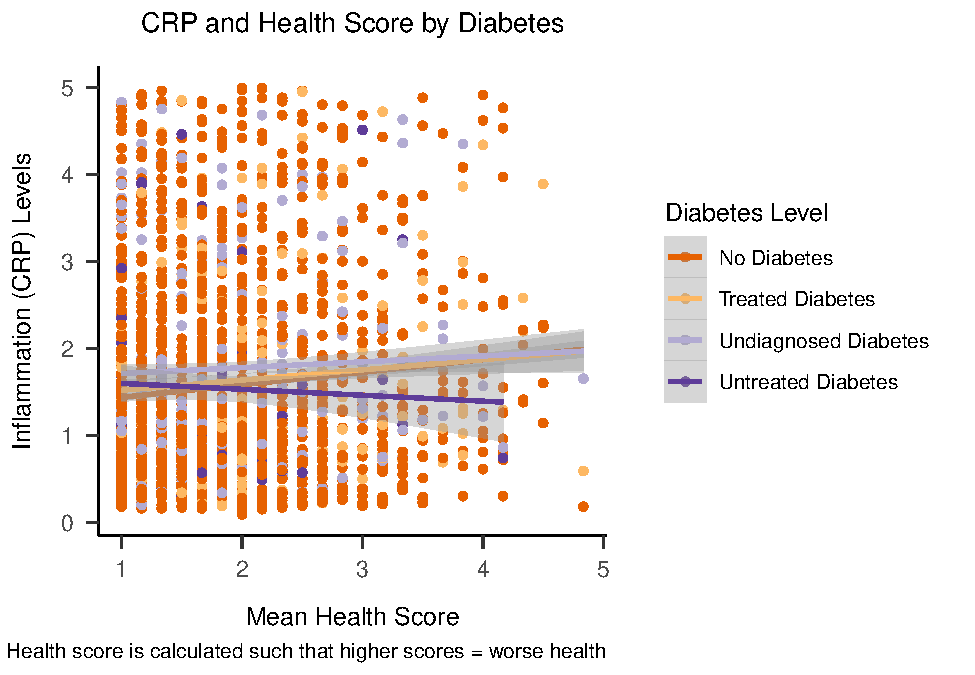
\includegraphics{NEW_Final_Groupof5_files/figure-latex/appendix-fig1-1.pdf}
\caption{\label{fig:appendix-fig1}Here goes the caption.}
\end{figure}





\begin{figure}
\centering
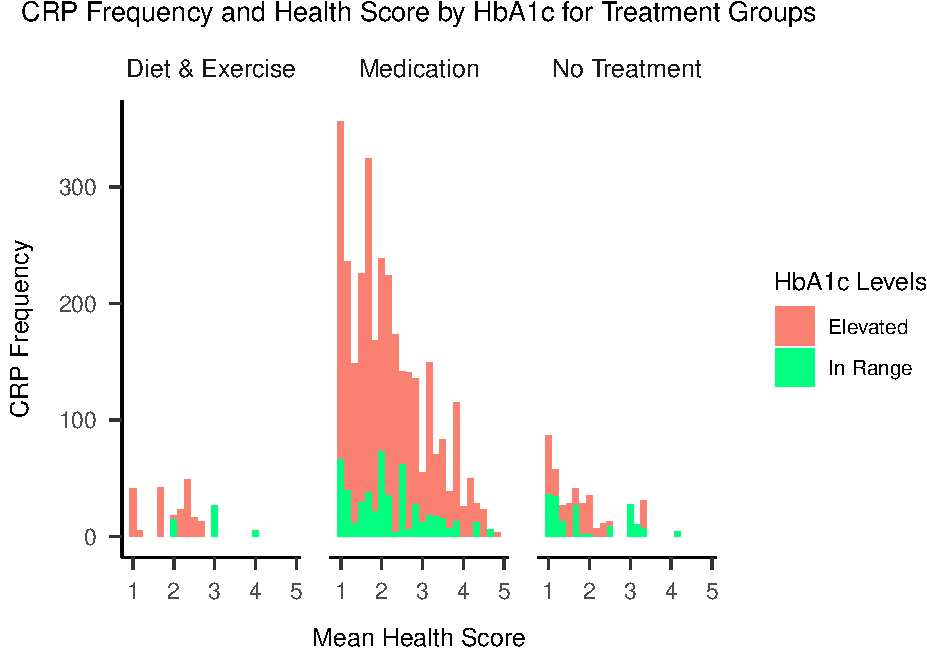
\includegraphics{NEW_Final_Groupof5_files/figure-latex/appendix-fig3-1.pdf}
\caption{\label{fig:appendix-fig3}Here goes the caption.}
\end{figure}



\begin{figure}
\centering
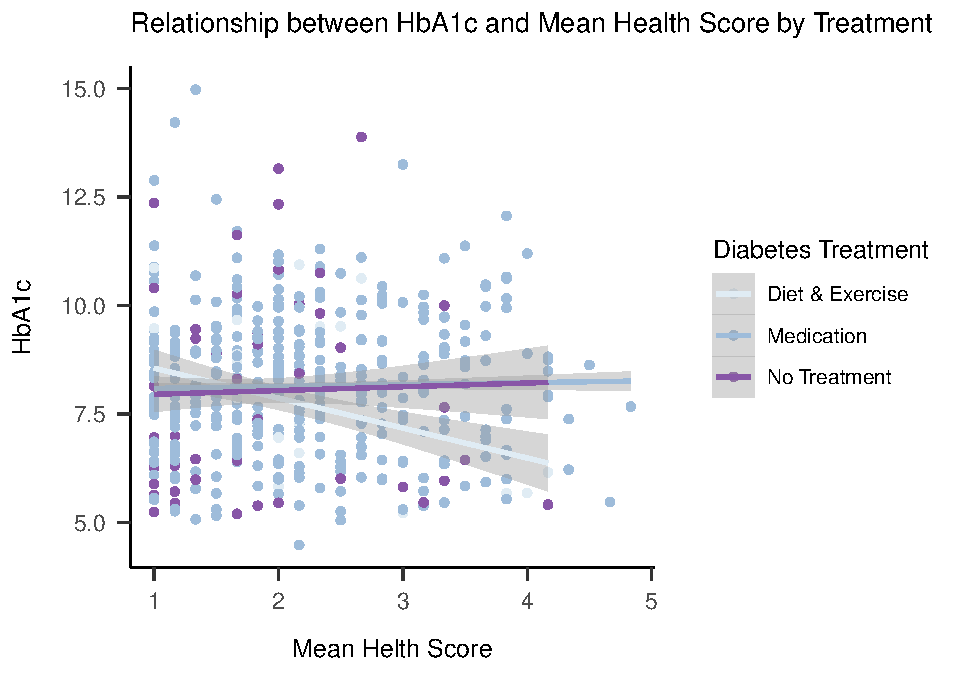
\includegraphics{NEW_Final_Groupof5_files/figure-latex/appendix-fig4-1.pdf}
\caption{\label{fig:appendix-fig4}Here goes the caption.}
\end{figure}





\begin{longtable}[]{@{}
  >{\raggedright\arraybackslash}p{(\columnwidth - 4\tabcolsep) * \real{0.0541}}
  >{\raggedright\arraybackslash}p{(\columnwidth - 4\tabcolsep) * \real{0.3243}}
  >{\raggedright\arraybackslash}p{(\columnwidth - 4\tabcolsep) * \real{0.6216}}@{}}
\caption{\label{tab:descriptives} Descriptive statistics.}\tabularnewline
\toprule()
\begin{minipage}[b]{\linewidth}\raggedright
\end{minipage} & \begin{minipage}[b]{\linewidth}\raggedright
\end{minipage} & \begin{minipage}[b]{\linewidth}\raggedright
Mexico
\end{minipage} \\
\midrule()
\endfirsthead
\toprule()
\begin{minipage}[b]{\linewidth}\raggedright
\end{minipage} & \begin{minipage}[b]{\linewidth}\raggedright
\end{minipage} & \begin{minipage}[b]{\linewidth}\raggedright
Mexico
\end{minipage} \\
\midrule()
\endhead
\(N_{total}\) & & 357 \\
Sex & & \\
& male & 115 (32.20 \%) \\
& female & 241 (67.50 \%) \\
& unknown & 1 (0.30 \%) \\
Age & & 68 (\(SD\) = 8.40) \\
\bottomrule()
\end{longtable}

\begin{figure}
\centering
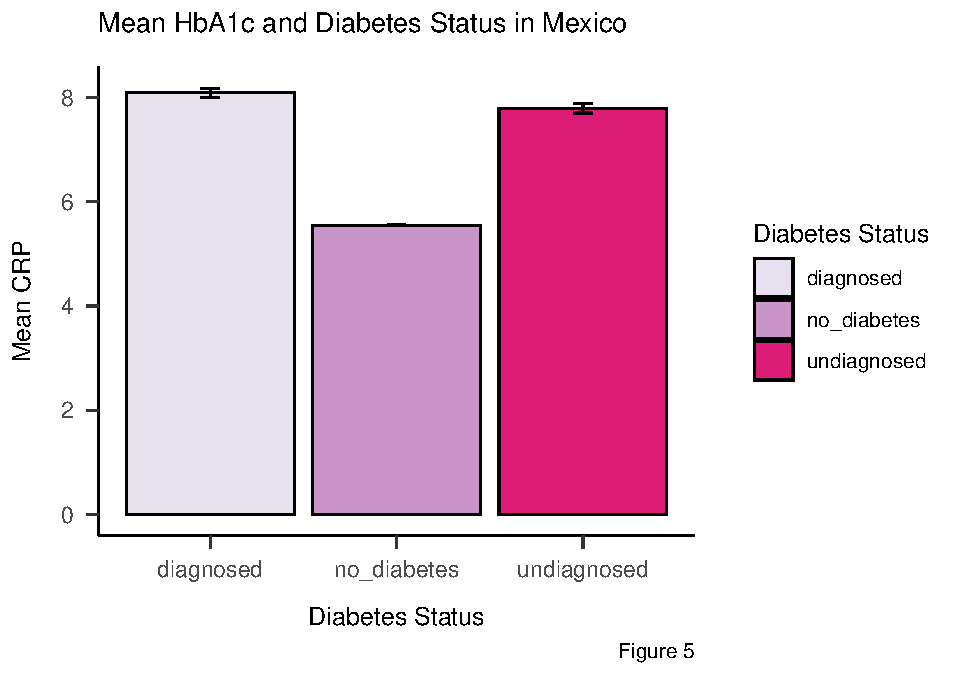
\includegraphics{NEW_Final_Groupof5_files/figure-latex/dshba1c-1.pdf}
\caption{\label{fig:dshba1c}Here goes the caption.}
\end{figure}



\begin{figure}
\centering
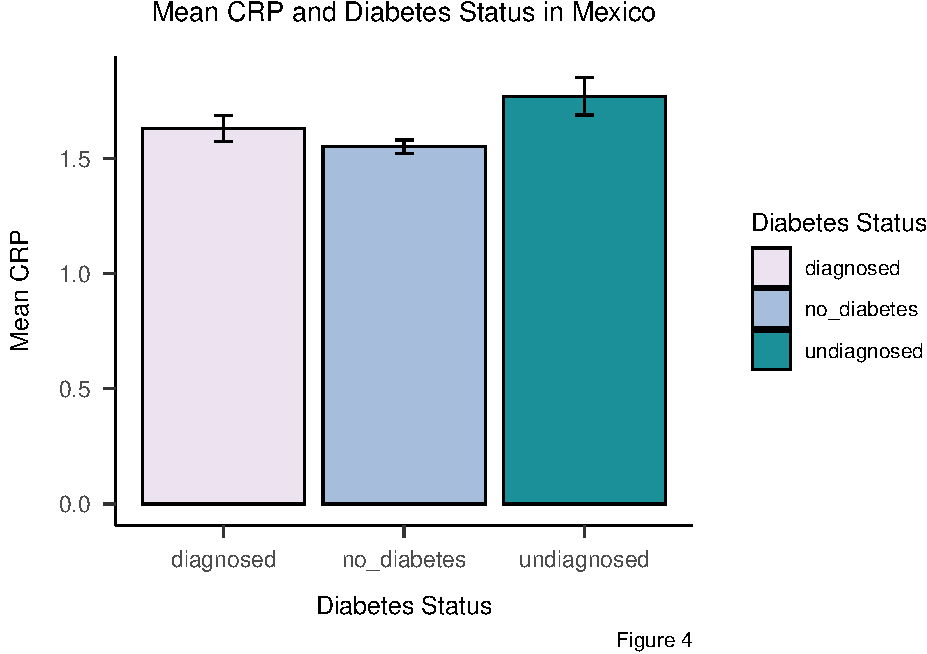
\includegraphics{NEW_Final_Groupof5_files/figure-latex/dscrp-1.pdf}
\caption{\label{fig:dscrp}Here goes the caption.}
\end{figure}



\begin{figure}
\centering
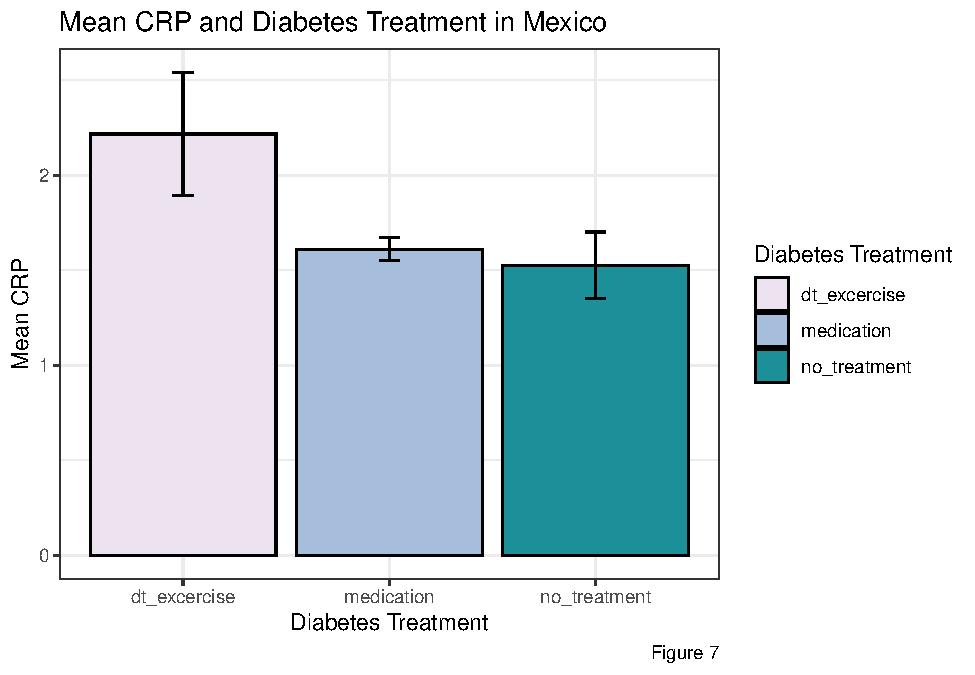
\includegraphics{NEW_Final_Groupof5_files/figure-latex/treat-fig-1.pdf}
\caption{\label{fig:treat-fig}Here goes the caption.}
\end{figure}



\hypertarget{introduction}{%
\section{Introduction}\label{introduction}}

Diabetes and its insidious complications continue to expand as a global health burden at an alarming rate. In 2021, there were approximately 537 million adults living with diabetes in the world and this number is expected to jump to 783 million by 2045. A disproportionate percentage of these people live in low to middle income countries (LMICs). Given this predicted jump in incidence and in light of the COVID-19 pandemic, there is a heightened need in better understanding diabetes. During COVID-19, diabetes was found to both increase the severity of COVID-19 symptoms (in people with elevated a1c levels) and increase in incidence (\protect\hyperlink{ref-yangPrevalenceComorbiditiesIts2020}{Yang et al., 2020}) (\protect\hyperlink{ref-rohmInflammationObesityDiabetes2022}{Rohm, Meier, Olefsky, \& Donath, 2022}). Additionally, diabetes is associated with a steep increase in cardiovascular disease risk and is a leading cause of death in many low to middle income countries (LMICs) including Mexico.

Although the precise classification of diabetes remains controversial because of the complex nature of its pathogenesis, there are three universally acknowledged subtypes: type 1 diabetes, type 2 diabetes, and gestational diabetes. Diabetes is a progressive disease in that the longer one has it, the more complications ensue. Therefore, it is helpful to conceptualize diabetes as a process that can be stopped, but not reversed. Research that contributes to slowing down or stopping the process can be extremely valuable to global health regardless of its contribution to cure and prevention because of the astronomical rates of diabetes in our world today.

Research shows that inflammation predicts the development of diabetes and is found to be a strong indicator of diabetes development and progression.(\protect\hyperlink{ref-freemanCreactiveProteinIndependent2002}{Dilys J. Freeman et al., 2002}) (\protect\hyperlink{ref-10.1161ux2f01.cir.103.3.357}{Dilys J. Freeman et al., 2001}) (\protect\hyperlink{ref-schmidtMarkersInflammationPrediction1999}{Schmidt et al., 1999}). Specifically, trials for drugs directed at inflammation among people with type 2 diabetes have indicated that drugs targeted at inflammation may be a therapeutic option for preventing diabetes (\protect\hyperlink{ref-10.4239ux2fwjd.v5.i5.697}{Agrawal \& Kant, 2014}). In addition, retinopathy and focal neuropathy (\protect\hyperlink{ref-saidDiabeticNeuropathyReview2007}{Said, 2007}) have also been linked to inflammatory processes. Conversely, when left untreated, the direct damage caused by high blood glucose leads to more inflammation and creates a nasty feedback loop wherein inflammation causes more insulin resistance which leads to high blood glucose. Furthermore, it has been found that the ability of cells to absorb insulin can be increased through diet, exercise, and oral pills.

A current gap in literature exists investigating the relationship between inflammation levels and the different treatments offered to those with diabetes, such as diet, exercise, and medication. This study seeks to fill this gap by investigating the extent to which inflammation levels relate to medication and diet and exercise among older Mexicans with diabetes.

\hypertarget{methods}{%
\section{Methods}\label{methods}}

\hypertarget{data}{%
\subsection{Data}\label{data}}

To examine the extent to which inflammation relates to medication, diet, and exercise among older Mexicans, we performed secondary data analyses using the two datasets from from the Wave 1 Study on Global Ageing (SAGE) from the World Health Organization (WHO). Cross-sectional baseline data was originally collected in 2016 through in-person interviews lasting on average between 90-120 minutes among Mexicans (age range) in Mexico.

\hypertarget{procedures-and-sample}{%
\subsection{Procedures and Sample}\label{procedures-and-sample}}

357 participants were included in our analyses. Of those, 115 were assessed to be male (32.20 \%), 241 were identified to be female (67.50 \%). Sex data for 1 participant was missing (see Table \ref{tab:descriptives}). This indicates that females were overrepresented in our sample, assuming binary sexes are represented equally in the population (\(\chi^2\)(1) = 44.60, \(p\) \textless{} 0.0001). The age in our sample was \(M\) = 68 years (SD = 8.40 years).
Because of missing values in the variables of interest in some of our analyses, subjects were excluded. Thus, \(N\) is reported separately for each analysis.

\hypertarget{variables}{%
\subsection{Variables}\label{variables}}

The original WHO dataset contains more than 1,600 variables, not all of which are relevant to our research questions. Therefore, we have limited our analysis to 10 variables, listed below in Table 1. In our analysis, we only included participants who reported that they already have a formal diabetes diagnosis from a doctor, since our research questions revolve around diabetes treatments. Figure (plot\_all) shows the raw data and the data that we selected for our analysis (the colorful points on the far left).

\hypertarget{filtering}{%
\subsubsection{Filtering}\label{filtering}}

A variable was created called ``diabetes treatment'' that indicated whether or not someone fell into one of the three following categories: medication, diet and exercise, and no treatment.Anyone who answered yes to ``Have you been taking insulin or other blood sugar lowering medications in the last 2 weeks?'' was coded ``yes'' for medication. Anyone who answered yes to ``Have you been following a special diet, exercise regime or weight control program for diabetes during the last 2 weeks?'' was coded yes for diet and exercise. Anyone who answered no to both was coded as ``no treatment''. A variable was then created that indicated ``unknown treatment'' if the diabetes treatment variable indicated that there was no treatment but hba1c was below 6.5 and otherwise ``Known treatment'' was indicated. All ``unknown treatment'' variables were then removed (n = 17). See plot.all2 and plot.all\_filtered to see the data before and after these data points were filtered out.

\hypertarget{biomarkers}{%
\subsubsection{Biomarkers}\label{biomarkers}}

Biomarkers.A subset of people participating in the SAGE study underwentbiomarker analysis in Mexico (n = 1831) and in China (n = 12,077). Exclusions included 194 people for having an elevated CRP value that might indicate injury or infection. The sample was 60\% female and 40\% male. Participant ages for this analysis ranged from 50 to 105 years old (M = 68.27, SD = 9.23).

Biomarkers were analyzed using dried blood spot (DBS) procedures, and collected via standard venipuncture into an EDTA tube. In order to go from venous blood to DBS, the samples of whole blood were homogenized and then pipetted in 20uL aliquots onto standard Whatman 903 filter paper. The samples were left to dry for 24 hours at room temperature before they were analyzed. We punched out a 6mm spot from the DBS card and used 250 uL of PBS buffer pH = 7 to elute for 14 hours. The Abbott Architect CI8200 chemistry analyzer was used to analyzed the DBS eluates in order to obtain CRP values and it was used for HbA1c as well.

Hemoglobin A1c (HbA1c) is a measure of average blood glucose values over the past 3 months. HbA1c also required a 6 mm DBS punch. This one was eluted in 400uL MULTIAGEN Hemoglobin Denaturant for 14 hours. The Architect blood chemistry analyzer was loaded with a cuvette with eluent and was then used to determine HbA1c and total hemoglobin by measuring absorbance at 700 for Hba1cnm and 604nm for total hemoglobin. The analyzer's program calculated percent HbA1c using the following formula:{[}(HbA1c/TotHb)×100{]} - 3+(0.2 × TotHb).

Self-report surveys conducted by trained interviewers.

Data are from the World Health Organization's Study on Adult Health and Ageing (SAGE). Our data is from 1 of 5 countries where the data were collected.

All analyses were conducted in R with the following packages:
here (\protect\hyperlink{ref-here}{Müller, 2020}), rio(\protect\hyperlink{ref-chanRioSwissarmyKnife2021a}{Chan, Chan, Leeper, \& Becker, 2021}), tidyverse{[}re{]}, ggpubr (\protect\hyperlink{ref-kassambaraGgpubrGgplot2Based2022}{Kassambara, 2022}),bibtex (\protect\hyperlink{ref-francoisBibtexBibtexParser2022}{Francois \& Hernangómez, 2022}),papaja (\protect\hyperlink{ref-austPapajaPrepareReproducible2022}{Aust \& Barth, 2022}), psych
(\protect\hyperlink{ref-revellePsychProceduresPsychological2022}{Revelle, 2022}),and forcats (\protect\hyperlink{ref-wickhamForcatsToolsWorking2022}{Wickham, 2022}), janitor(\protect\hyperlink{ref-firkeJanitorSimpleTools2021}{Firke, 2021}), gt (\protect\hyperlink{ref-iannoneGtEasilyCreate2022}{Iannone, Cheng, Schloerke, Hughes, \& Seo, 2022}), stargazer(\protect\hyperlink{ref-hlavacStargazerWellformattedRegression2018}{Hlavac, 2018}).

\hypertarget{results}{%
\section{Results}\label{results}}

We see the expected relationships between diabetes status and HbA1c (see Figure \ref{fig:dshba1c}). However, with CRP we see a relatively similar level of CRP between people without diabetes and those with diagnosed diabetes (see Figure \ref{fig:dscrp}). Thus, we explored whether medication may be responsible for lowering CRP. In Figure \ref{fig:treat-fig} we see that those who are using diet and exercise as treatment have higher CRP levels than those taking medication and those not on treatment. We explored this further statistically.

\hypertarget{regression-1}{%
\subsection{Regression 1}\label{regression-1}}

For our first research question, does taking medication lower inflammation levels, we found that this regression model (Table \ref{tab:regtab1}) using 357 participants was not significant \(F\)(2, 354) = 1.06, \(p\) = 0.35 with \(R^2\) = 0.01. The regression coefficient for age was \(b_{age}\) = -0.01 (\(SE\) = 0.01, \(p\) = 0.36), and for use of medication \(b_{medication}\) = 0.20 (\(SE\) = 0.18, \(p\) = 0.28). Therefore, based on these results we fail to reject our null hypothesis and we cannot conclude that there is a relationship between medication and inflammation levels on average in this population.

\hypertarget{regression-2}{%
\subsection{Regression 2}\label{regression-2}}

Our research question two looked at diet and exercise as a treatment for diabetes on predicting inflammation levels. We found that this regression model (Table \ref{tab:RQ2}) using 357 participants was not significant \(F\)(2, 354) = 2.70, \(p\) = 0.07 with \(R^2\) = 0.01. The regression coefficient for age was \(b_{age}\) = -0.01 (\(SE\) = 0.01, \(p\) = 0.41), and for diet and exercise \(b_{Diet}\) = -0.24 (\(SE\) = 0.12, \(p\) \textless{} 0.05). Based on these results, fail to reject our null hypothesis and conclude that diet and exercise does not predict inflammation levels on average in this population.

\hypertarget{chi-square-test}{%
\subsection{Chi Square Test}\label{chi-square-test}}

To gain insight into the relation between accessing health care and the treatment option: diet and exercise among those with diabetes partaking we conducted a Chi-square test of independence. Based on this analysis there were no significant differences in those utilizing care in the last year (Y/N) and partaking in diet and exercise (Y/N). In addition, to evaluate whether accessing health care in the last year relates with inflammation levels among those that partake in diet and exercise only, we conducted another chi-square test of independence. Results for this analysis were also not significant.

To better understand differences in outcomes in health among those partaking in diet and exercise versus those that are not to treat diabetes, we seek to understand if there is difference in those that accessed health care in the last year and those that use diet and exercise as a treatment option for diabetes. \(\chi^2\) results: (\(\chi^2\)(1) = 0.57, \(p\) = 0.45). Based on these results we fail to reject the null hypothesis, and cannot conclude seeing a doctor in the last year relates to individuals using diet and exercise as treatment for diabetes in this population sample.

Looking at individuals who partake in diet and exercise only as a treatment for diabetes, we seek to answer the extent to which seeing a doctor in the last year relates to inflammation levels. \(\chi^2\) results: (\(\chi^2\)(1) = 0.57, \(p\) = 0.45). Based on these results, we fail to reject our null hypothesis and cannot conclude that seeing a doctor in the last year relates to inflammation levels in this population sample.

\hypertarget{discussion}{%
\section{Discussion}\label{discussion}}

We see diet and exercise predicting CRP over and above the effects of age such that those who said that they do diet and exercise have higher CRP.

Ultimately we see that inflammation is impacted by diabetes treatments. Access to care does not appear to explain this relationship. However, it is important that further exploration between diabetes, inflammation, and diabetes treatments take place.

\hypertarget{limitations}{%
\subsection{Limitations}\label{limitations}}

Among the different treatment options for diabetes, medication can mean either pills or insulin. There are different implications for these representative treatment options for inflammation and diabetes. However, we were not able to look at pills and insulin separately, or medication combinations, and some of their effects have the potential to cancel each other out.Given that we do not know exactly which medication people were taking, combination therapy is a possibility we could not account for. In addition, the sex variable was established through interviewer discernment and was not self reported.

Because data analyzed are from cross-sectional studies only, we cannot infer causality and there are likely many factors that account for significant differences in inflammation levels among older Mexicans.

\newpage

\hypertarget{appendix}{%
\section{Appendix}\label{appendix}}

Despite the documented limitations of the World Health Organization Health State Description scale (\protect\hyperlink{ref-asadaMedicalTechnologiesNonhuman2005}{Asada, 2005}), it is worth exploring in future studies whether or not this scale captures diabetes complications in such a way that we might be able to analyze connections between inflammation and diabetes complications cross-sectionally in the SAGE data.

\newpage

\hypertarget{references}{%
\section{References}\label{references}}

\hypertarget{refs}{}
\begin{CSLReferences}{1}{0}
\leavevmode\vadjust pre{\hypertarget{ref-10.4239ux2fwjd.v5.i5.697}{}}%
Agrawal, N. K., \& Kant, S. (2014). Targeting inflammation in diabetes: {Newer} therapeutic options. \emph{World Journal of Diabetes}, \emph{5}(5), 697. \url{https://doi.org/10.4239/wjd.v5.i5.697}

\leavevmode\vadjust pre{\hypertarget{ref-asadaMedicalTechnologiesNonhuman2005}{}}%
Asada, Y. (2005). Medical technologies, nonhuman aids, human assistance, and environmental factors in the assessment of health states. \emph{Quality of Life Research}, \emph{14}(3), 867--874. \url{https://doi.org/10.1007/s11136-004-0910-z}

\leavevmode\vadjust pre{\hypertarget{ref-austPapajaPrepareReproducible2022}{}}%
Aust, F., \& Barth, M. (2022). \emph{{papaja}: {Prepare} reproducible {APA} journal articles with {R Markdown}}. manual. Retrieved from \url{https://github.com/crsh/papaja}

\leavevmode\vadjust pre{\hypertarget{ref-chanRioSwissarmyKnife2021a}{}}%
Chan, C., Chan, G. C., Leeper, T. J., \& Becker, J. (2021). \emph{Rio: {A Swiss-army} knife for data file {I}/{O}}. manual.

\leavevmode\vadjust pre{\hypertarget{ref-firkeJanitorSimpleTools2021}{}}%
Firke, S. (2021). \emph{Janitor: {Simple} tools for examining and cleaning dirty data}. manual. Retrieved from \url{https://CRAN.R-project.org/package=janitor}

\leavevmode\vadjust pre{\hypertarget{ref-francoisBibtexBibtexParser2022}{}}%
Francois, R., \& Hernangómez, D. (2022). \emph{Bibtex: {Bibtex} parser}. manual. Retrieved from \url{https://CRAN.R-project.org/package=bibtex}

\leavevmode\vadjust pre{\hypertarget{ref-freemanCreactiveProteinIndependent2002}{}}%
Freeman, Dilys J., Norrie, J., Caslake, M. J., Gaw, A., Ford, I., Lowe, G. D. O., \ldots{} Study, W. of S. C. P. (2002). C-reactive protein is an independent predictor of risk for the development of diabetes in the west of scotland coronary prevention study. \emph{Diabetes}, \emph{51}(5), 1596--1600. \url{https://doi.org/10.2337/diabetes.51.5.1596}

\leavevmode\vadjust pre{\hypertarget{ref-10.1161ux2f01.cir.103.3.357}{}}%
Freeman, Dilys J., Norrie, J., Sattar, N., Neely, R. D. G., Cobbe, S. M., Ford, I., \ldots{} Gaw, A. (2001). Pravastatin and the development of diabetes mellitus. \emph{Circulation}, \emph{103}(3), 357--362. \url{https://doi.org/10.1161/01.cir.103.3.357}

\leavevmode\vadjust pre{\hypertarget{ref-hlavacStargazerWellformattedRegression2018}{}}%
Hlavac, M. (2018). \emph{Stargazer: {Well-formatted} regression and summary statistics tables}. manual, {Bratislava, Slovakia}: {Central European Labour Studies Institute (CELSI)}. Retrieved from \url{https://CRAN.R-project.org/package=stargazer}

\leavevmode\vadjust pre{\hypertarget{ref-iannoneGtEasilyCreate2022}{}}%
Iannone, R., Cheng, J., Schloerke, B., Hughes, E., \& Seo, J. (2022). \emph{Gt: {Easily} create presentation-ready display tables}. manual. Retrieved from \url{https://CRAN.R-project.org/package=gt}

\leavevmode\vadjust pre{\hypertarget{ref-kassambaraGgpubrGgplot2Based2022}{}}%
Kassambara, A. (2022). \emph{Ggpubr: 'ggplot2' based publication ready plots}. manual. Retrieved from \url{https://CRAN.R-project.org/package=ggpubr}

\leavevmode\vadjust pre{\hypertarget{ref-here}{}}%
Müller, K. (2020). \emph{Here: {A} simpler way to find your files}. manual. Retrieved from \url{https://CRAN.R-project.org/package=here}

\leavevmode\vadjust pre{\hypertarget{ref-revellePsychProceduresPsychological2022}{}}%
Revelle, W. (2022). \emph{Psych: {Procedures} for psychological, psychometric, and personality research}. manual, {Evanston, Illinois}: {Northwestern University}. Retrieved from \url{https://CRAN.R-project.org/package=psych}

\leavevmode\vadjust pre{\hypertarget{ref-rohmInflammationObesityDiabetes2022}{}}%
Rohm, T. V., Meier, D. T., Olefsky, J. M., \& Donath, M. Y. (2022). Inflammation in obesity, diabetes, and related disorders. \emph{Immunity}, \emph{55}(1), 31--55. \url{https://doi.org/10.1016/j.immuni.2021.12.013}

\leavevmode\vadjust pre{\hypertarget{ref-saidDiabeticNeuropathyReview2007}{}}%
Said, G. (2007). Diabetic neuropathy---a review. \emph{Nature Clinical Practice Neurology}, \emph{3}(6, 6), 331--340. \url{https://doi.org/10.1038/ncpneuro0504}

\leavevmode\vadjust pre{\hypertarget{ref-schmidtMarkersInflammationPrediction1999}{}}%
Schmidt, M. I., Duncan, B. B., Sharrett, A. R., Lindberg, G., Savage, P. J., Offenbacher, S., \ldots{} Heiss, G. (1999). Markers of inflammation and prediction of diabetes mellitus in adults ({Atherosclerosis Risk} in {Communities} study): A cohort study. \emph{The Lancet}, \emph{353}(9165), 1649--1652. \url{https://doi.org/10.1016/S0140-6736(99)01046-6}

\leavevmode\vadjust pre{\hypertarget{ref-wickhamForcatsToolsWorking2022}{}}%
Wickham, H. (2022). \emph{Forcats: {Tools} for working with categorical variables (factors)}. manual. Retrieved from \url{https://CRAN.R-project.org/package=forcats}

\leavevmode\vadjust pre{\hypertarget{ref-yangPrevalenceComorbiditiesIts2020}{}}%
Yang, J., Zheng, Y., Gou, X., Pu, K., Chen, Z., Guo, Q., \ldots{} Zhou, Y. (2020). Prevalence of comorbidities and its effects in patients infected with {SARS-CoV-2}: A systematic review and meta-analysis. \emph{International Journal of Infectious Diseases}, \emph{94}, 91--95. \url{https://doi.org/10.1016/j.ijid.2020.03.017}

\end{CSLReferences}

\newpage

\hypertarget{tables-and-figures}{%
\section{Tables and Figures}\label{tables-and-figures}}


\clearpage
\renewcommand{\listfigurename}{Figure captions}

\clearpage
\renewcommand{\listtablename}{Table captions}


\end{document}
